\section{Experiments}
\label{sec:exps}
In this section, we will conduct experiments to examine the following hypotheses: (1) DASC can achieve strong controllability while also preserving good generation quality in multi-attribute controllable generation. (2) Both the learned meaningful representations in the attribute semantic space, and the reasonable parameter amount benefit DASC's performance. (3) DASC can also be flexibly extended for other control tasks like the composition of multiple emotions or adopting certain strategies for emotional support. 

\subsection{Experiment Settings}
% \subsubsection{Data}
We conduct experiments on the \textit{self} split of the DuLemon dataset~\citep{xu2022long}, which is a Chinese open-domain dialogue dataset that is rich in personalized content so that we can find the various attributes we would like to control. We split the data to train/dev/test set with 352999, 2439, 2412 utterances each. Since the original dataset do not contain annotations of control attributes, we leverage automatic methods to label the dataset. For gender style (male, female, neutral), we use the dataset released by \citet{su2020stylistic} to train a MacBERT classifier, which achieved accuracy=94.98\%. For emotion, we follow \citet{zhou2018emotional} and use the NLPCC2013 and NLPCC2014 dataset (8 emotion classes) to train another MacBERT classifier, which has an accuracy of 93.96\%. For the question dialogue act (question VS non-question), we simply use a heuristic for labeling: if the sentence contains a question mark(?) we will consider it a question and otherwise non-question. We then use these 3 methods to assign each response in the dataset with the 3 aspects of attributes (13 in total). 
% \KZ{For Chinese, many people omit question marks when typing a question.}
% \ZL{In this dataset, we find most questions will use a question mark. But there do exist be cases where question ends with a period(。). This only consists of a small fraction (about 3%) so will not constitute a big problem.}

\subsubsection{Compared Methods}
We compare the proposed DASC framework with representative methods from different types of controllable generation methods. We use the \texttt{fnlp/bart-base-chinese} \citep{shao2021cpt} model as the backbone for all compared methods.

\paragraph{Baseline} Simply fine-tuning the backbone on the dataset without utilizing the control attributes.

\paragraph{Rerank} Using top-$p$ sampling \citep{holtzman2019curious} on the baseline model to produce 5 response candidates for each context, and attribute classifiers (here are the same separate models we've used for auto-annotations) to rerank the candidates. Following \citet{thoppilan2022lamda}, we use the sum of predicted probabilities in each aspect for ranking. 

\paragraph{CTRL} We re-implemented \citet{keskar2019ctrl}'s method for dialogue generation by defining 3 groups of special control codes for each aspect, and appending the corresponding 3 attribute tokens to each dialogue context during fine-tuning.

\paragraph{Director} The multi-attribute extension of Director \citep{arora2022director} discussed in \secref{sec:weighted_decoding}. 

All models are fine-tuned on the dataset for 6 epochs, and the decoding method is top-$p$ sampling with $p=0.5$. Director and DASC use control weight $\alpha=1$ and classifier loss weight $\beta=0.1$. When conducting multi-aspect control for Director and DASC under weighted-decoding paradigm (\eqnref{eqn:multi_wd_logits}), we set the variables for the desired attribute as 1, and other variables as $\phi$.  

\subsubsection{Evaluation}
\paragraph{Automatic Evaluation} To evaluate the controllability, we use the same attribute classifiers as those used for labeling the dataset to calculate the accuracy of attributes in the generation (Acc$_G$, Acc$_E$, Acc$_Q$ for gender, emotion and question, respectively). For the generation quality, we use BertScore (BScore) \cite{zhang2019bertscore} to evaluate generation's similarity to reference response, and Distinct-2 \cite{li2016diversity} for diversity. 

\paragraph{Human Judgement} We sampled 100 contexts from the test set for human evaluation. Since the distribution of the original test set is extremely skewed, we've specified a constraint for more balanced distribution over all emotions during sampling, so as to ensure the representativeness of the evaluation (21 none, 16 sadness, 16 disgust, 16 happiness, 16 like, 5 anger, 5 surprise, 5 fear). We invited 2 volunteers who are proficient in Chinese to evaluate each generation from 3 perspectives. \textbf{Attribute Accuracy}: if the response conveys the given attribute. \textbf{Sensibleness}$_{(1-4)}$: if the response is fluent, coherent with the context, and accords with commonsense. \textbf{Interestingness}$_{(1-4)}$: whether the response is specific, novel and can encourage more interesting conversation continuation. The annotators have gone through extensive training to understand the requirements of the evaluation. We've also provided guidelines on our annotations UI, so that they can follow them throughout the course.

\subsection{Results}
\label{sec:results}
\begin{table}[]
    \small
    \centering
    \begin{tabular}{rccccc}
    \hline
             & BScore      & Dist-2         & Acc$_G$         & Acc$_E$         & Acc$_Q$          \\ \hline
    Baseline & 68.18          & 19.25          & 68.49          & 46.31          & 69.61           \\
    Rerank   & 69.23          & 19.28          & 75.46          & 54.93          & 82.42           \\
    CTRL     & \textbf{71.09} & 18.91          & 85.32          & 77.49          & \textbf{100.00} \\
    Director & 69.54          & {\ul 21.40}    & {\ul 95.81}    & \textbf{86.73} & \textbf{100.00} \\
    DASC     & {\ul 70.42}    & \textbf{21.94} & \textbf{95.85} & {\ul 86.07}    & \textbf{100.00} \\ \hline
    \end{tabular}
    \caption{Automatic evaluation results on DuLemon test set. The best results are in bold, while the second results are underlined.}
    \label{tab:auto_results}
\end{table}

Automatic evaluation results are shown in Table \ref{tab:auto_results}. We can see that the Rerank method failed to show strong controllability because the base model struggles to produce attributed ranking candidates without finetuning with the control attributes. The CTRL model leveraged the attributes in finetuning, and achieved better control accuracy and BertScore, but it doesn't produce more diverse responses overall. Both Director and DASC exhibit the best controllability, and DASC produces more diverse and reasonable responses according to Distinct-2 and BertScore. 

\begin{table}[]
    \small
    \centering
    \begin{tabular}{rccccc}
    \hline
                & Acc$_G$       & Acc$_E$       & Acc$_Q$  & Interest      & Sensible      \\ \hline
    Baseline & 0.80          & 0.55          & 0.64          & 2.04          & \textbf{3.46} \\
    Rerank   & 0.81          & 0.62          & 0.82          & 2.13          & 3.44          \\
    CTRL     & 0.85          & 0.82          & \textbf{0.97} & 2.24          & \textbf{3.46} \\
    Director & 0.87          & 0.87          & 0.96          & 2.25 & 3.26 \\
    DASC     & \textbf{0.88} & \textbf{0.88} & \textbf{0.97} & \textbf{2.37} & 3.28 \\ \hline
    \end{tabular}
    \caption{Human Judgement on DuLemon test set.}
    \label{tab:human_results}
\end{table}

We then show human judgement results in Table \ref{tab:human_results}. The inter-annotator agreement for Acc$_G$, Acc$_E$ and Acc$_Q$ are 0.65, 0.55 and 0.64 in Cohen's $\kappa$, which indicates moderate to substantial agreement. The agreement of $Interestingness$ and $Sensibleness$ is 0.48 and 0.44 in Pearson's $r$. The evaluation on attribute accuracies is similar to the automatic results, except that the accuracy of gender slightly decreases as human evaluators don't take neutral content that fits common gender prototypes as correctly reflecting the gender style, like soldier for male and baby-carer for female \citep{bolukbasi2016man}. The annotators also check questions without a question mark, which explains the slight difference in Acc$_Q$.

Overall, the rankings of controllability still hold according to human evaluation, with DASC performs the best. Baseline, Rerank and CTRL have slightly better \textit{Sensibleness} than weighted decoding methods, which agrees with the commonly observed controllability-quality trade-off in previous literature \citep{dathathri2019plug,yang2021fudge,qian2022controllable}. All controllable generation methods achieved higher \textit{Interestingness} score than baseline, which supports the benefits of controllable generation. DASC achieved the best \textit{Interestingness} given similar attributes accuracy as Director, indicating the effectiveness of attribute semantic space, which can establish better representations of attribute semantics and a more reasonable approach to compose the control attributes in weighted decoding. 

% \KZ{The results above don't seem to support the claim that DASC or attribute
% space has advantage over the naive extension of Director to m-Director in
% Sec. 2.3. This is a weakness.}
% \ZL{The advantage is more significant in Robustness Test (DASC avoids degeneration) and Parameter Analysis (M-Director suffers from over-parameterization)}

\subsection{Robustness Test}
In previous experiments, the control attributes provided to the model come from the reference response. Therefore, models may coincidentally hit the desired attributes when generating the most likely response to the context, without truly reliable controllability for arbitrary given attributes. Hence, we further conduct experiments to test the robustness of the controllable generation methods in out-of-distribution scenarios. 

Specifically, we sampled 100 contexts from the test set, and give the models each of the 8 emotions as the generation condition, paired with the original gender and question act\footnote{We do not change these 2 attributes as they are sometimes determined given the context.}. We then use greedy decoding to generate response for each \(context, attributes\) pair and conduct similar automatic and human evaluation on the 800 generations. 

\begin{table}[th]
    \small
    \centering
    \begin{tabular}{rcccc}
    \hline
             & Dist-2         & Acc$_E$            & Interest      & Sensible      \\ \hline
    Rerank   & 17.55          & 17.00          & -             & -             \\
    CTRL     & 21.07          & 43.38          & 1.91          & \textbf{3.00} \\
    Director & \textit{34.73} & 61.88          & 1.62          & 2.27             \\
    DASC     & \textbf{26.71} & \textbf{65.38} & \textbf{2.08} & 2.82 \\ \hline
    \end{tabular}
    \caption{Robustness test results.}
    \label{tab:robustness}
\end{table}

\begin{figure*}[t]
    \centering
    \begin{subfigure}{}
        \centering
        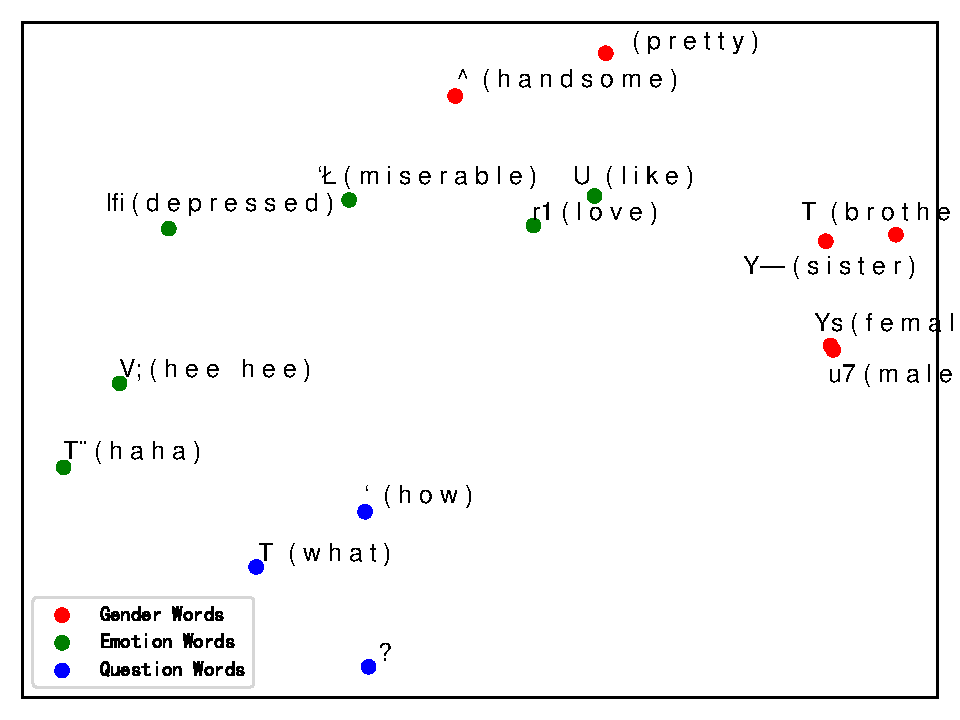
\includegraphics[width=.48\linewidth]{figures/tsne_sub_plot_token_emb2.pdf}  
    \end{subfigure}
    \begin{subfigure}{}
        \centering
        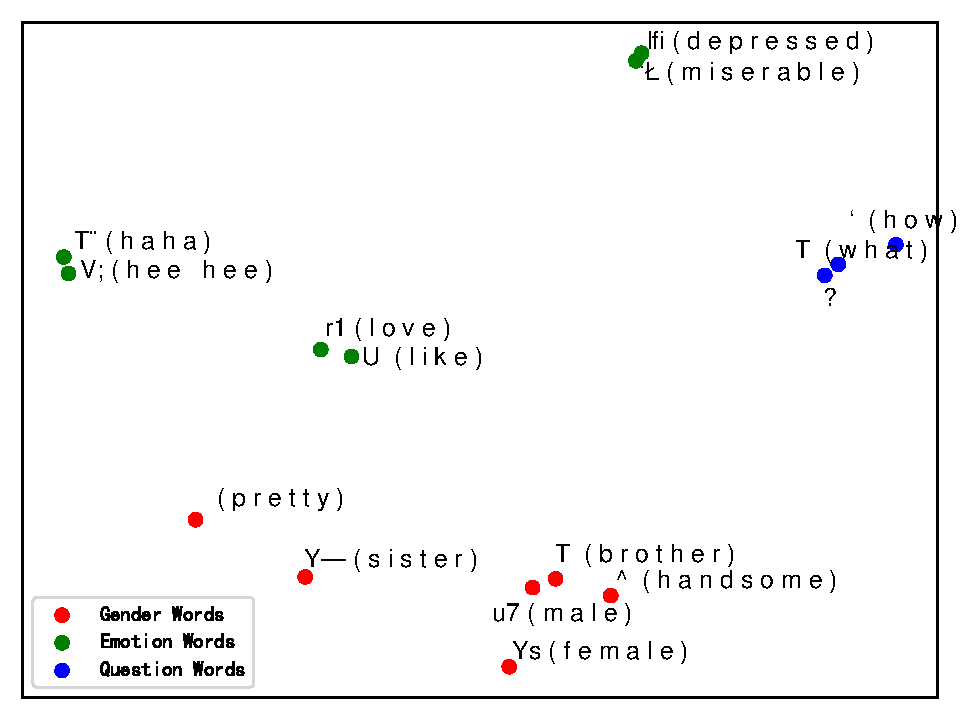
\includegraphics[width=.48\linewidth]{figures/tsne_sub_plot2.pdf}  
    \end{subfigure}
    \caption{Comparison of two sets of token embeddings with t-SNE visualization: those from the language model (left) and from the attribute semantic space (right).}
    \label{fig:token_emb}
\end{figure*}

\begin{figure}[t]
    \centering
    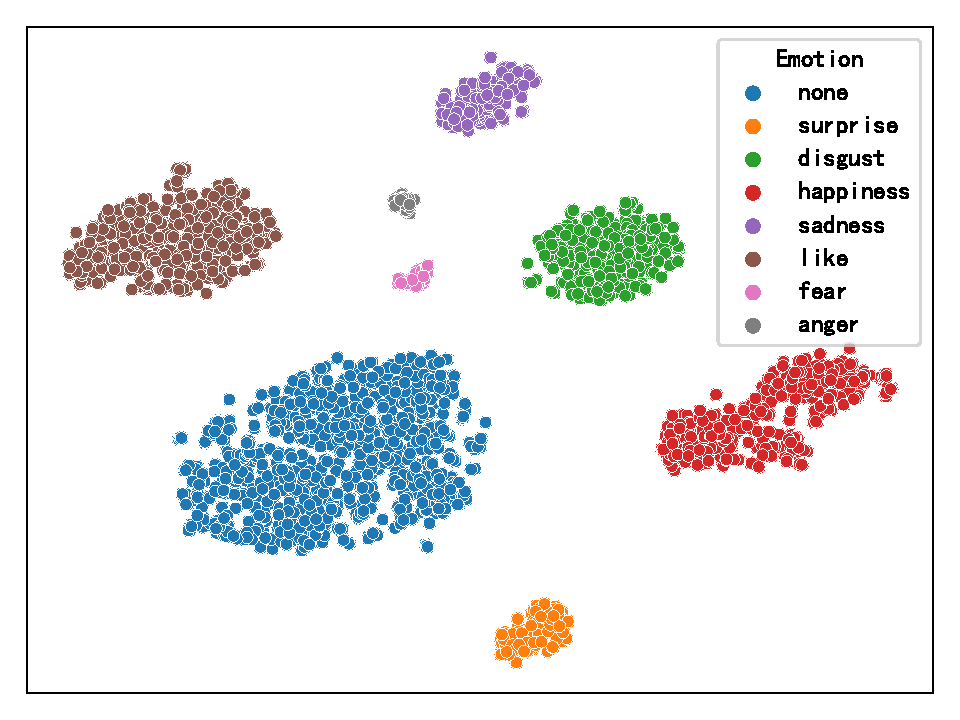
\includegraphics[width=1.0\columnwidth]{figures/emotion_context_emb.pdf}
    \caption{The t-SNE visualization of attribute context embedding of responses with different emotions.}
    \label{fig:emotion_context_emb}
\end{figure}

Table \ref{tab:robustness} shows the robustness test results.\footnote{BertScore is not reported here, as the model can be directed towards attributes different from the ground truth, invalidating the similarity-based metric as a proxy for generation quality.} Compared with Table \ref{tab:auto_results}, we can see that the emotion accuracy of Rerank and CTRL dropped significantly, which shows that their controllability is not generalizable. Another notable phenomenon is the abnormal \textit{Distinct-2} achieved by Director. We then further analyze their performance with human evaluation (excluding Rerank as it fails to control attributes). We found that Director frequently generate ungrammatical, illogical and repetitive long responses (like the second response in Figure \ref{fig:teaser_example}). Director's loss in emotion accuracy is also higher than DASC, indicating that it may overfit the training distribution given its large parameters, and thus performs worse in this out-of-distribution setting. Compared to CTRL, DASC has lower \textit{Sensibleness} but higher \textit{Interestingness}, when it also has a significant advantage in diversity and controllability. 


\subsection{Space Visualization}

For a clear understanding of how the proposed attribute semantic space can help controllable generation, we visualize them in 2D space with t-SNE \citep{van2008visualizing}. First, we visualize the attribute token embeddings of some representative attribute-related tokens, and also compare them with the corresponding embedding in the original LM (Figure \ref{fig:token_emb}). Comparing the two figures, we can see that (1) The token embeddings from different aspects are more separable in the attribute space (see points with different colors), while tokens in the same aspect are closes despite the difference in other linguist features like part-of-speech (like `handsome' and `male'). (2) The token embeddings from different attributes of the same aspect are also distinguished in the attribute space (like `male'-`female', `love'-`miserable'). These characteristics of the learned attribute space enable DASC to successfully control the generation of distinctive attributes and compose attributes from different aspects.


Next, we also visualize the attribute context embedding. Specifically, we take the responses with certain attribute in the dev set of the dataset, feed them into the model and average attribute context embeddings at each decoder token as sentence-level representations, and pair them with the sentence-level attribute annotations for analysis. For brevity, we only show the visualization with emotion labels in Figure \ref{fig:emotion_context_emb}, and provide those with gender and question act labels in Appendix. We can see that the context embeddings from sentences with different emotions are clearly separated in the space, which supports the strong controllability of DASC with multiple attributes.

\subsection{Parameter Analysis}
\label{sec:parameter_analysis}
% \KZ{It's very rare to use \S~ in scientific writing. It's mostly used in
% legal text. use the macros defined in acl2023.text for consistency.
% It's also not good to put figs or tables immediately below section
% headings. It's better to put them after you first refer to them.}
As analyzed in Sec. \ref{sec:dasc_method}, DASC can use a relatively smaller amount of parameters to implement weighted decoding for multi-attribute controllable generation. Here we study the effect of parameter numbers by adjusting the dimension of the attribute space $p$, and comparing with baseline and M-Director which uses no/large amount of parameters for attribute control respectively. We use BertScore to evaluate the generation quality and the average control accuracy on 3 aspects to reflect controllability.

\begin{table}[th]
    \small
    \centering
    \begin{tabular}{lccc}
    \hline
    Method      & \#params        & BScore         & Avg Acc        \\ \hline
    baseline    & -               & 68.18          & 61.47          \\
    DASC ($p$=512) & 15.94M          & 70.18          & 92.56          \\
    DASC ($p$=1024)& 31.88M          & 70.12          & 92.72          \\
    DASC ($p$=2048) & 63.75M          & \textbf{70.42} & 93.97          \\
    DASC ($p$=4096)& 127.50M         & 70.26          & \textbf{94.42} \\
    Director    & 210.98M         & 69.54          & 94.14          \\ \hline
    \end{tabular}
    \caption{Effect of the number of extra parameters for controllability and generation quality.}
    \label{tab:num_params}
\end{table}

Results are shown in Table \ref{tab:num_params}. Comparing DASC with different $p$, we can see that larger amount of parameters can generally improve the model's controllability, but even a relatively small $p$ ($p$=512) is already capable to achieve high control accuracy. For generation quality, a moderate number of parameters can achieve the best BertScore, but smaller ones do not significantly degrade the performance. Director, which additionally uses nearly twice the parameters of the base model (210.98M vs. 116.26M), may have been over-parameterized and thus harms its generation quality.

\subsection{Case Study}

Besides multi-aspect control as shown in Figure \ref{fig:teaser_example}, we also show a proof-of-concept application that DASC can naturally blend two emotions in one generated response. We can simply achieve this by setting both attributes' value as 1 instead of $\phi$. The results are shown in Figure \ref{fig:compose_example1_en} and Figure \ref{fig:compose_example2}. We can see that DASC can successfully generate responses with either single emotion or the combination of both emotions, where the later can produce potentially more vivid response.

\begin{figure}[t]
    \centering
    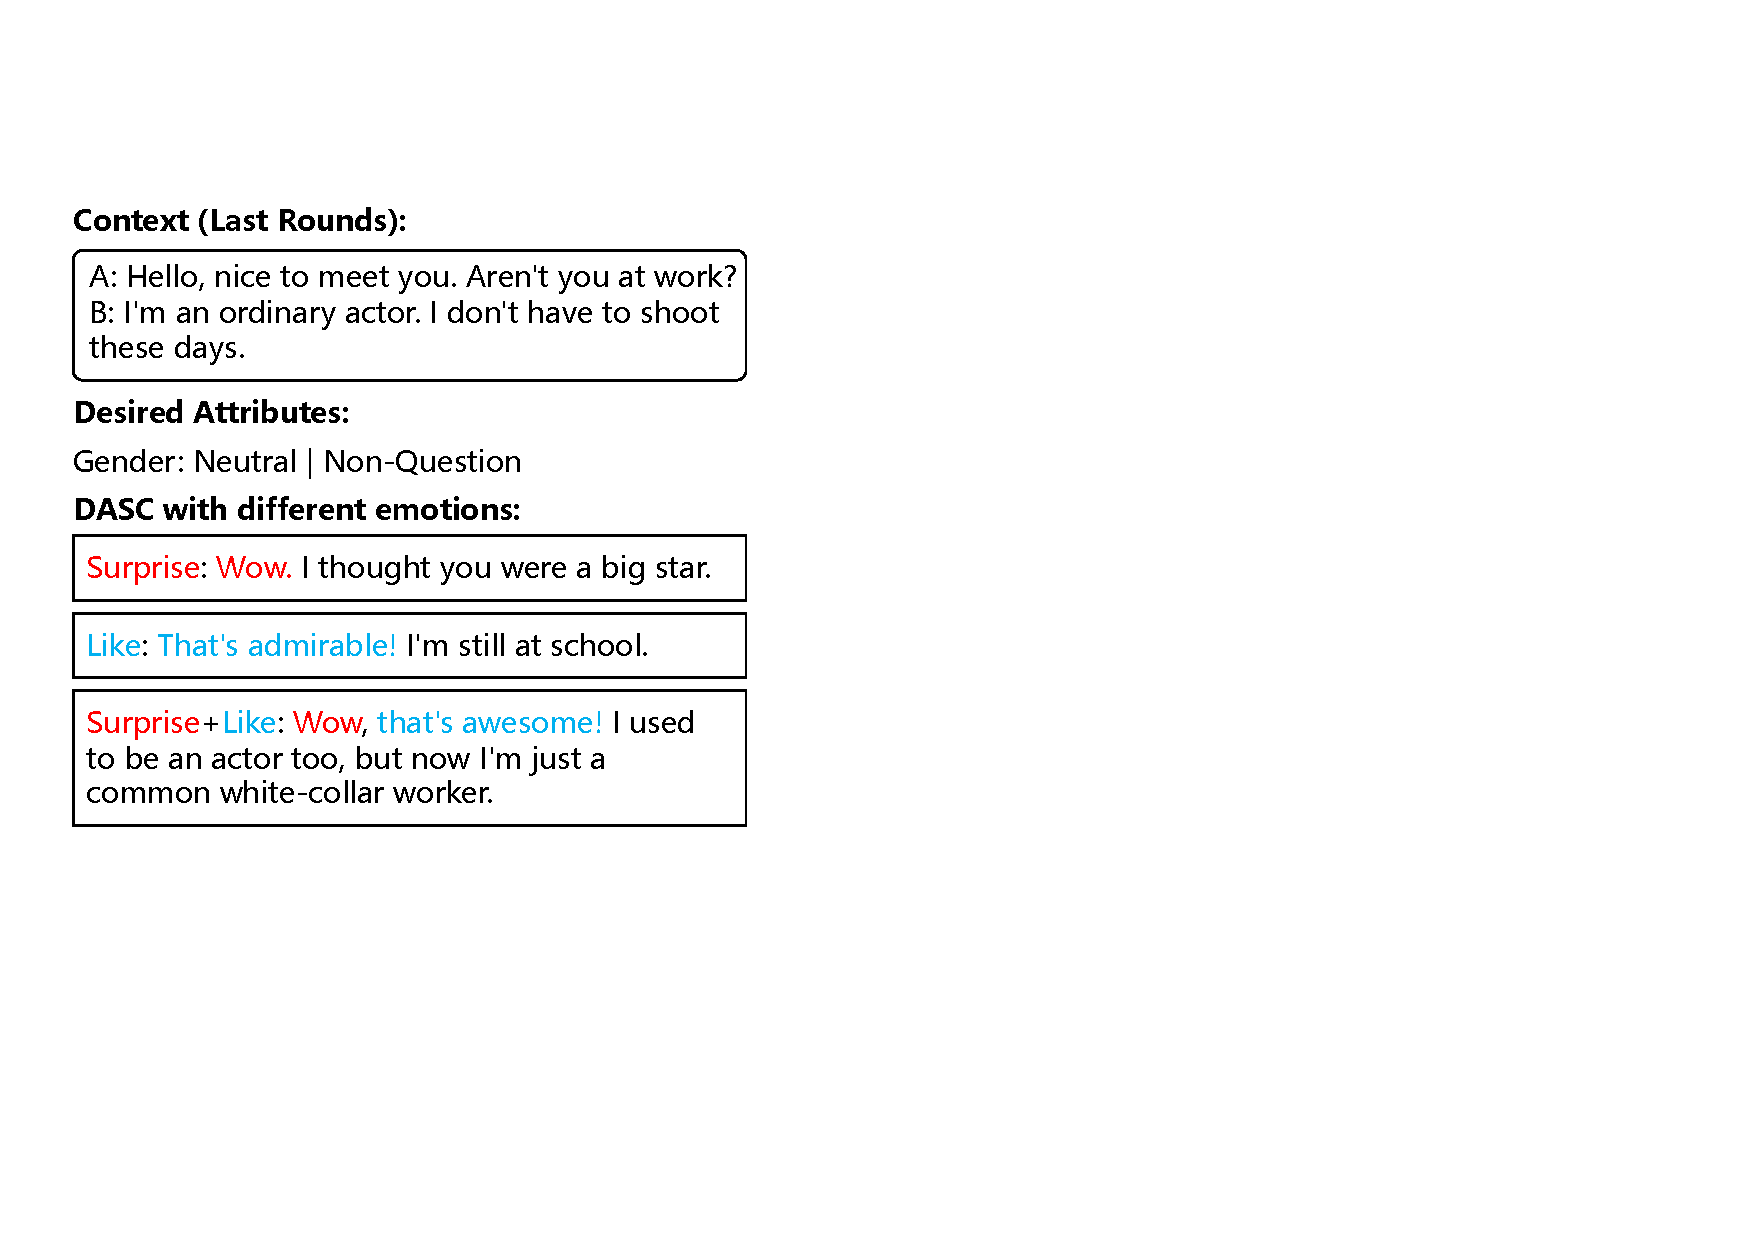
\includegraphics[width=1.0\columnwidth]{figures/compose_example1_en.pdf}
    \caption{DASC generates different responses to the same context given different emotions and their composition as control attributes. (Translated from Chinese, original text in Figure \ref{fig:compose_example1_zh})}
    \label{fig:compose_example1_en}
\end{figure}

\subsection{ESConv Experiment}

To further explore the potential of DASC, we also experimented on another dataset ESConv \citep{liu2021towards}. It is an English dataset that aims to provide emotional supports to help seekers with 8 defined strategies. Here we use the human annotated strategy labels as the control attributes, and experimented with 3 methods: \textbf{Baseline}, \textbf{CTRL} and \textbf{DASC}. We report the automatic metric \textbf{Distinct-2} and human evaluated \textbf{Strategy Accuracy}, \textbf{Usefulness}$_{(1-4)}$ and \textbf{Sensibleness}$_{(1-4)}$. In Table \ref{tab:esconv_results}, we can see that the control of relatively complex strategies is harder, and thus the accuracy is lower than the previous experiment (Table \ref{tab:human_results}). Nevertheless, DASC still achieves reasonable control accuracy and outperforms other methods on all metrics. These results suggest that DASC is language-agnostic and can be effectively applied to many kinds of attribute controls. We provide more details and generation examples in Appendix.

\begin{table}[th]
    \centering
    \small
    \begin{tabular}{rcccc}
        \hline
             & Dist-2         & Acc           & Useful        & Sensible      \\ \hline
    Baseline & 19.28          & 0.27          & 1.92          & 3.30          \\
    CTRL     & 21.20          & 0.52          & 2.04          & 3.31          \\
    DASC     & \textbf{25.86} & \textbf{0.70} & \textbf{2.24} & \textbf{3.48} \\ \hline
    \end{tabular}
    \caption{Test results on ESConv.}
    \label{tab:esconv_results}
\end{table}

